\section{SPH方法算例}

\subsection{文献中的算例}

\begin{frame}
    \begin{figure}[H]
        \centering
        \subfigure[水面兴波]{
            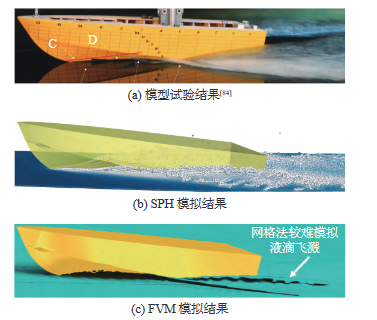
\includegraphics[width=0.3\textwidth]{images/xingbo.png}
        }
        \subfigure[细长体入水]{
            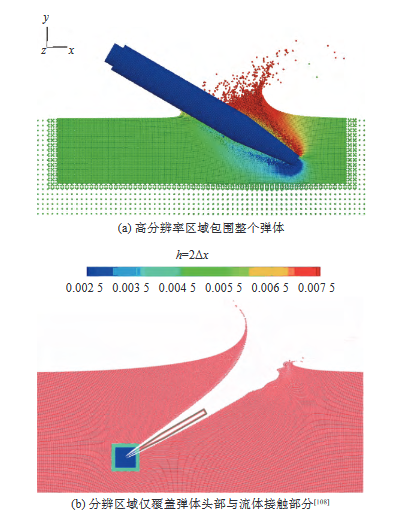
\includegraphics[width=0.25\textwidth]{images/xichangti.png}
        }\\
        \subfigure[水下爆炸]{
            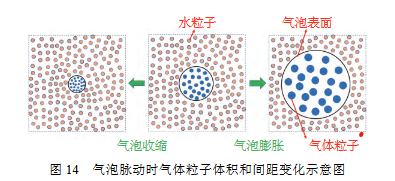
\includegraphics[width=0.5\textwidth]{images/shuixiabaozha.png}
        }
        \caption{SPH理论和方法在高速水动力学中的研究进展\cite{_sph_2022}}
    \end{figure}
\end{frame}

\begin{frame}
    \begin{figure}[H]
        \centering
        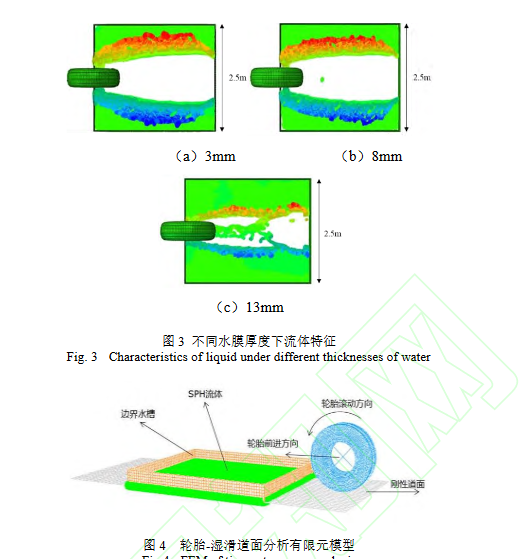
\includegraphics[width=0.6\textwidth]{images//luntai.png}
        \caption{飞机轮胎-湿滑道面相互作用SPH算法仿真分析\cite{_-sph_nodate}}
    \end{figure}
\end{frame}

\begin{frame}
        \begin{figure}[H]
            \centering
            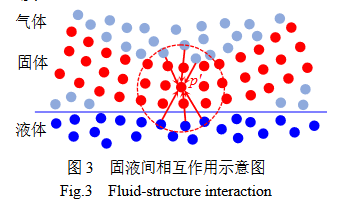
\includegraphics[width=0.6\textwidth]{images//tansuxing.png}
            \caption{基于改进光滑粒子流体动力学方法的弹塑性结构入水问题研究\cite{__nodate}}
        \end{figure}
\end{frame}

\begin{frame}
    \begin{figure}[H]
        \centering
        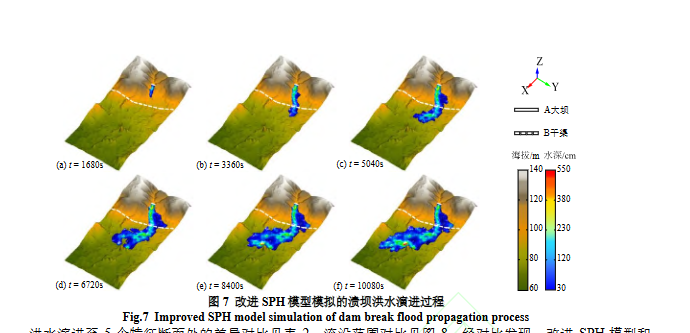
\includegraphics[width=0.6\textwidth]{images//kuibahongshui.png}
        \caption{基于改进SPH模型的溃坝洪水演进模拟方法\cite{_sph_nodate-2}}
    \end{figure}
\end{frame}

\begin{frame}
    \begin{figure}[H]
        \centering
        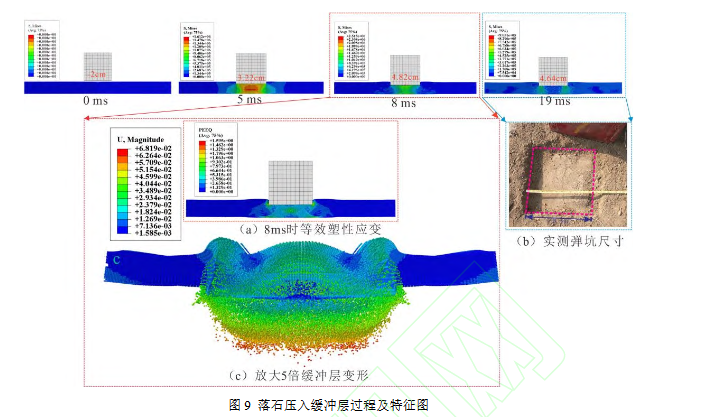
\includegraphics[width=0.6\textwidth]{images//ouhedabianxing.png}
        \caption{基于SPH-FEM的落石冲击缓冲层-钢筋混凝土板动力响应研究\cite{_sph-fem-_nodate}}
    \end{figure}
\end{frame}

\begin{frame}
    \begin{figure}[H]
        \centering
        \subfigure[粒子修正技术]{
            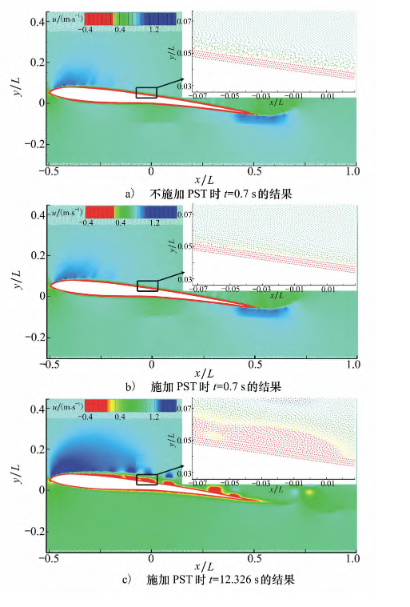
\includegraphics[width=0.2\textwidth]{images/lizixiuzheng.png}
        }\quad
        \subfigure[张力不稳定控制]{
            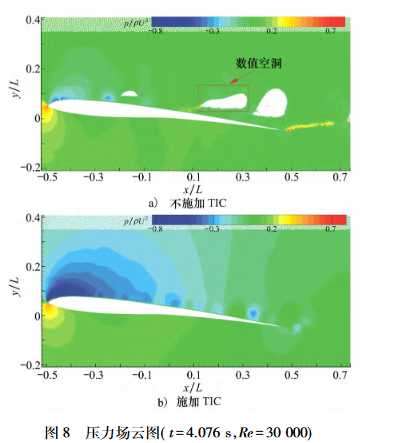
\includegraphics[width=0.25\textwidth]{images/zhanglibuwendingkongzhi.png}
        }\quad
        \subfigure[多级粒子分辨率技术与拉格朗日拟序结构]{
            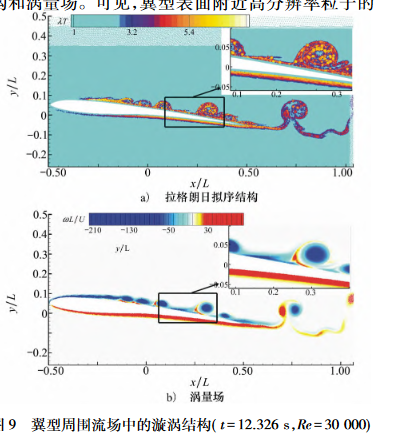
\includegraphics[width=0.25\textwidth]{images/duojilizi.png}
        }
        \caption{翼型绕流的多级分辨率光滑粒子流体动力学数值模拟研究\cite{__2022-3}}
    \end{figure}
\end{frame}

\subsection{SmoothedParticles.jl开源库算例}

\begin{frame}
    SmoothedParticles.jl是一个基于Julia语言的开源并行SPH库,
    其以Julia语言的高性能为基础,实现了SPH方法的核心算法,
    并将结果以Paraview的格式输出,方便后续的后处理。
    \begin{figure}[H]
        \centering
        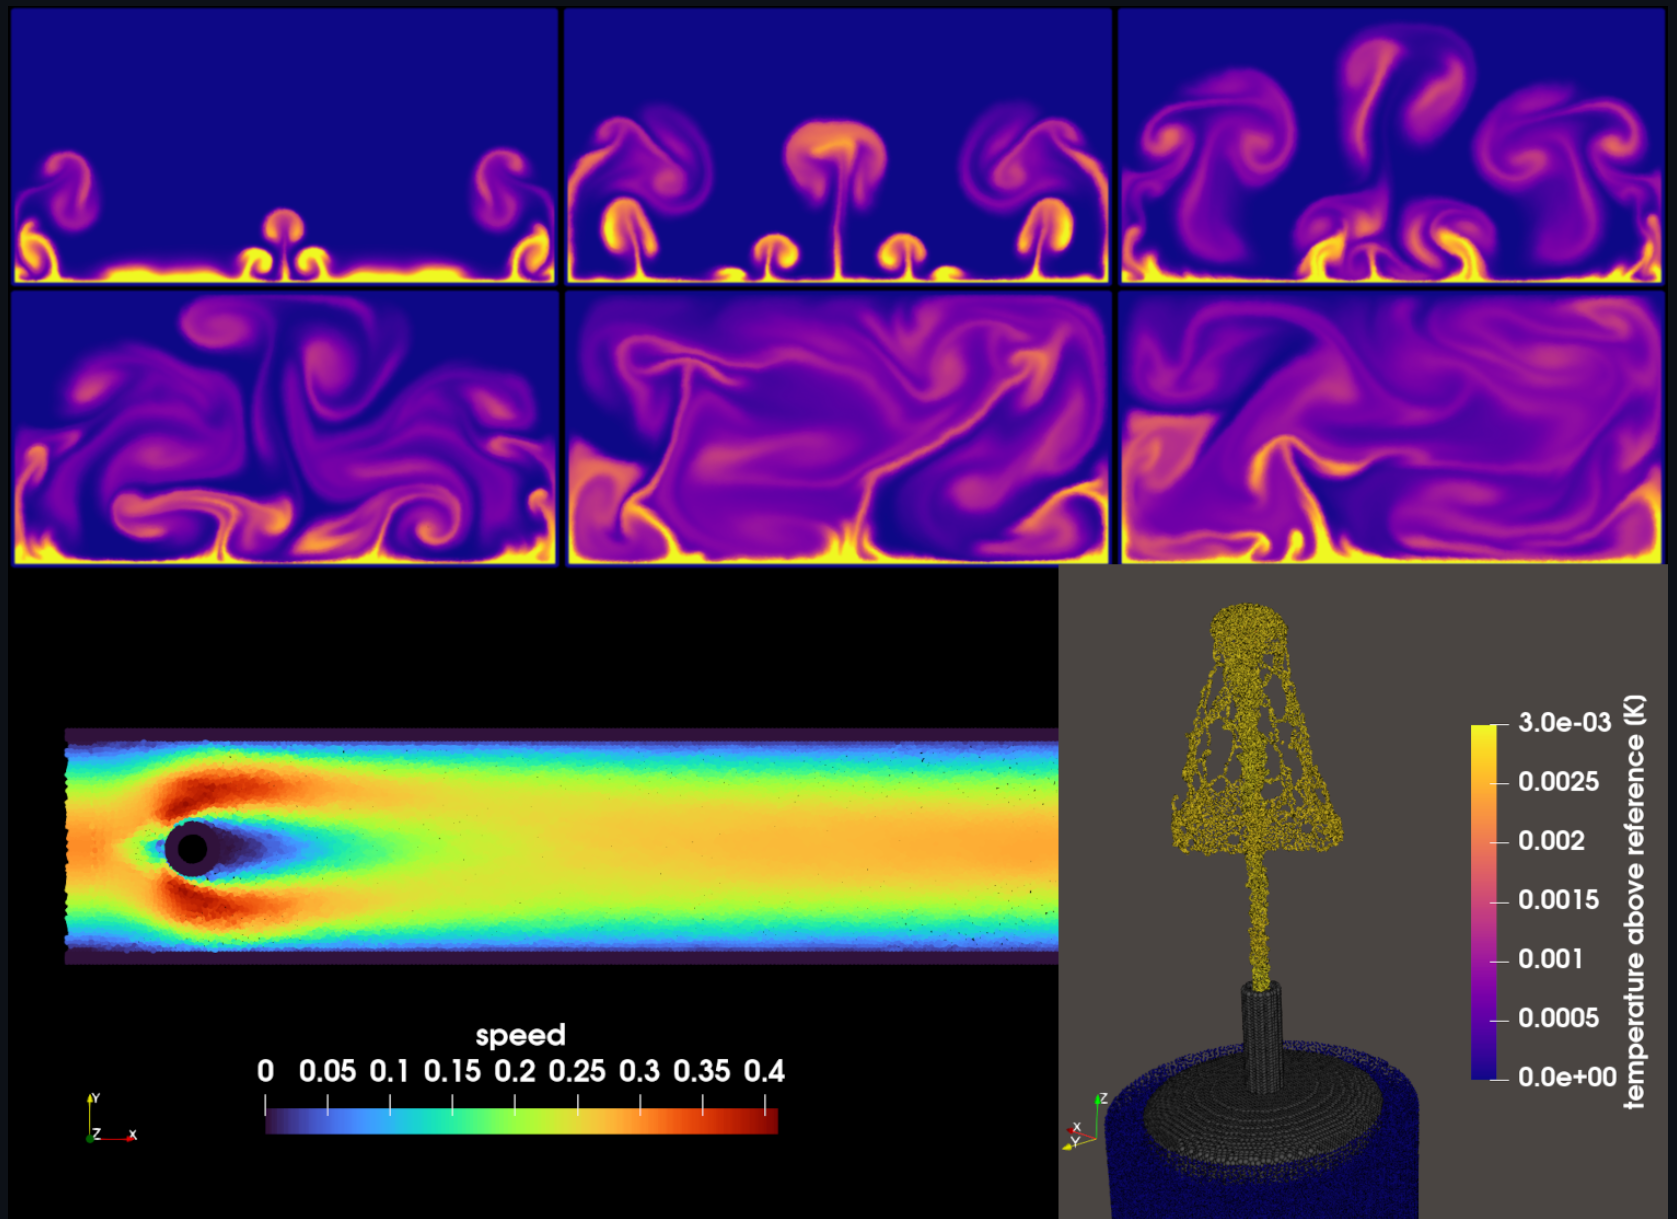
\includegraphics[width=0.6\textwidth]{images/smoothedparticles.png}
        \caption{SmoothedParticles.jl开源库}
    \end{figure}
\end{frame}

\begin{frame}

    \begin{figure}[H]
        \centering
        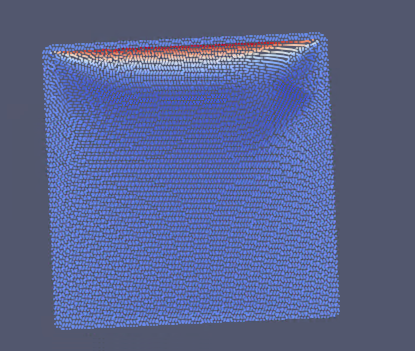
\includegraphics[width=0.6\textwidth]{images/lid_driven_cavity.png}
        \caption{顶盖驱动流算例}
    \end{figure}
\end{frame}

\begin{frame}
    \begin{figure}[H]
        \centering
        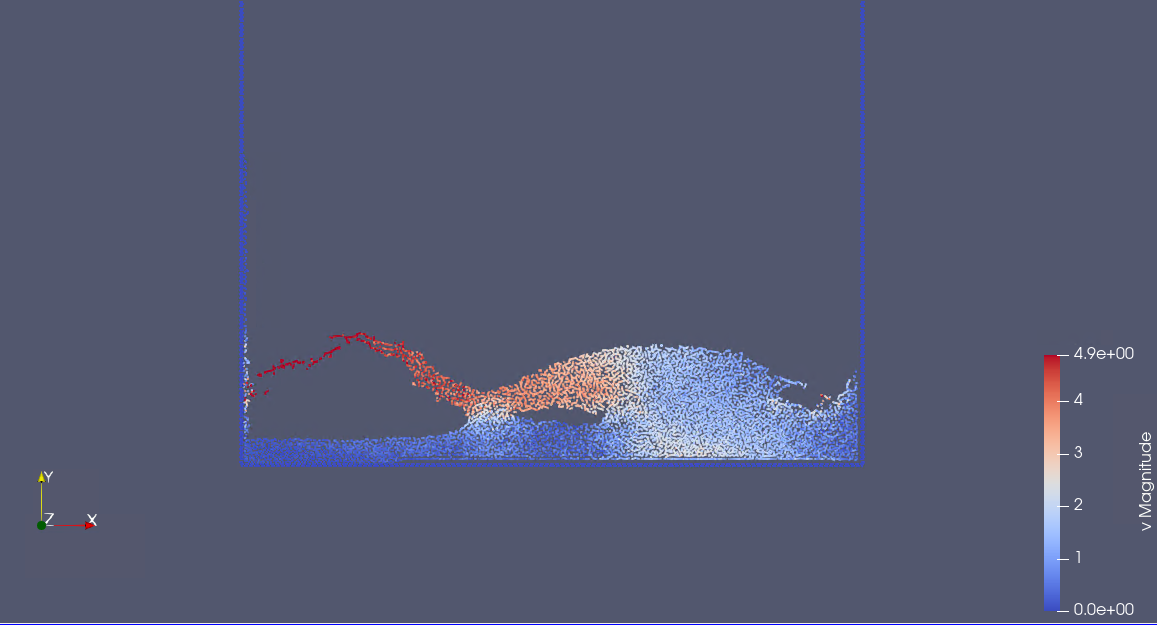
\includegraphics[width=0.6\textwidth]{images/free_surface.png}
        \caption{自由表面流}
    \end{figure}
    此算例用显示时间推进,计算了3000个粒子的运动,花费了40分钟。
\end{frame}

\begin{frame}
    \begin{figure}[H]
        \centering
        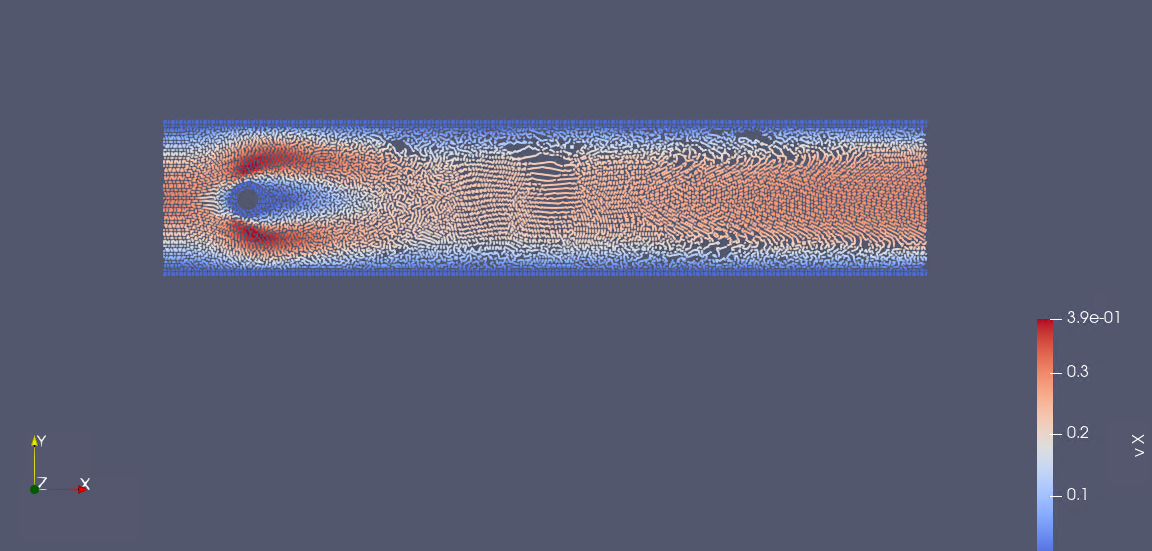
\includegraphics[width=0.6\textwidth]{images/cylindar.png}
        \caption{圆柱绕流}
    \end{figure}
\end{frame}